\documentclass{letter}

\usepackage[a4paper,margin=1in]{geometry}
\usepackage{graphicx}
\begin{document}

\setlength\parindent{24pt}
\date{\begin{flushleft}\today\end{flushleft}} % Use todays date and left-align it

\begin{letter}{\large \bfseries To: Mr. McLapply \\ From: David Lowe \\ Subject: Poisson Regression Simulation Study} 

\signature{
David Lowe \\
\textbf{Aspiring Statistician} \\ % Job title
}
\opening{Mr. McLapply,}

\fontsize{12pt}{14pt}\selectfont

It is difficult to derive a closed-form solution for the parameter, $\beta$, when using Poisson regression (see model below). The purpose of this study was to assess the accuracy and precision of various methods for estimating the parameter $\beta$. To do this I have developed several different methods for estimating $\hat{\beta}$. The first method employs a frequentist approach to estimate our parameter. I developed an estimator using the Wilk's method, Test-Inversion, and bootstrapping to estimate $\hat{\beta}$. I also approached the problem using Bayesian methods, with loss functions, 0-1, squared error, and absolute error loss. These were tested with both gaussian and uniform priors.

My simulation specifically analyzes the Wilk's method for calculating the MLE, the squared-error loss estimator with a $N(.4,.2)$ prior, and the 1-0 loss estimator with a $Unif(-5,5)$ prior. Each was estimated for several $\beta$ values ranging from 0 to 0.8. From these simulations I measured the bias and the mean squared error (MSE). 

From the results I observe that the mean squared error is very comparable between the different estimation methods. The trend shows that as $\beta$ increases, so does the mean squared error. The squared-error loss estimates have slightly higher MSE than Wilk's and 0-1 loss as $\beta$ nears 0, and again as it approaches 0.8. 

\begin{center}
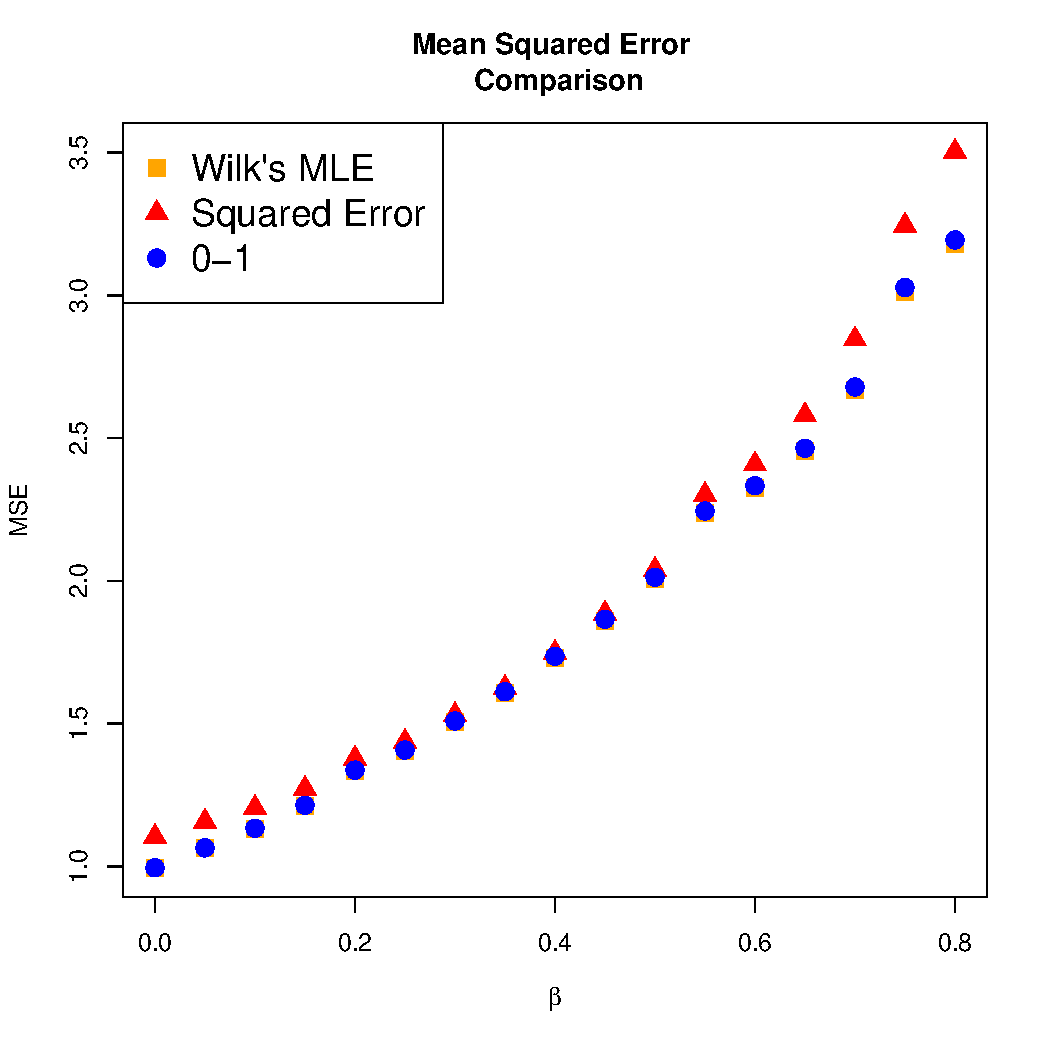
\includegraphics[scale=.45]{mse.pdf}
\end{center}

The simulations showed that bias did not have the same relationship between tests. Wilk's and squared-error loss methods perform similarly, with a negative bias at $\beta$ close to 0 and approaches a bias of 0 as they approach 0.8. 0-1 loss, however, shows a strong negative trend, from a positive bias to a negative as $\beta$ moves from 0 to 1, crossing the zero bias threshold at about $\beta=0.4$. 

\begin{center}
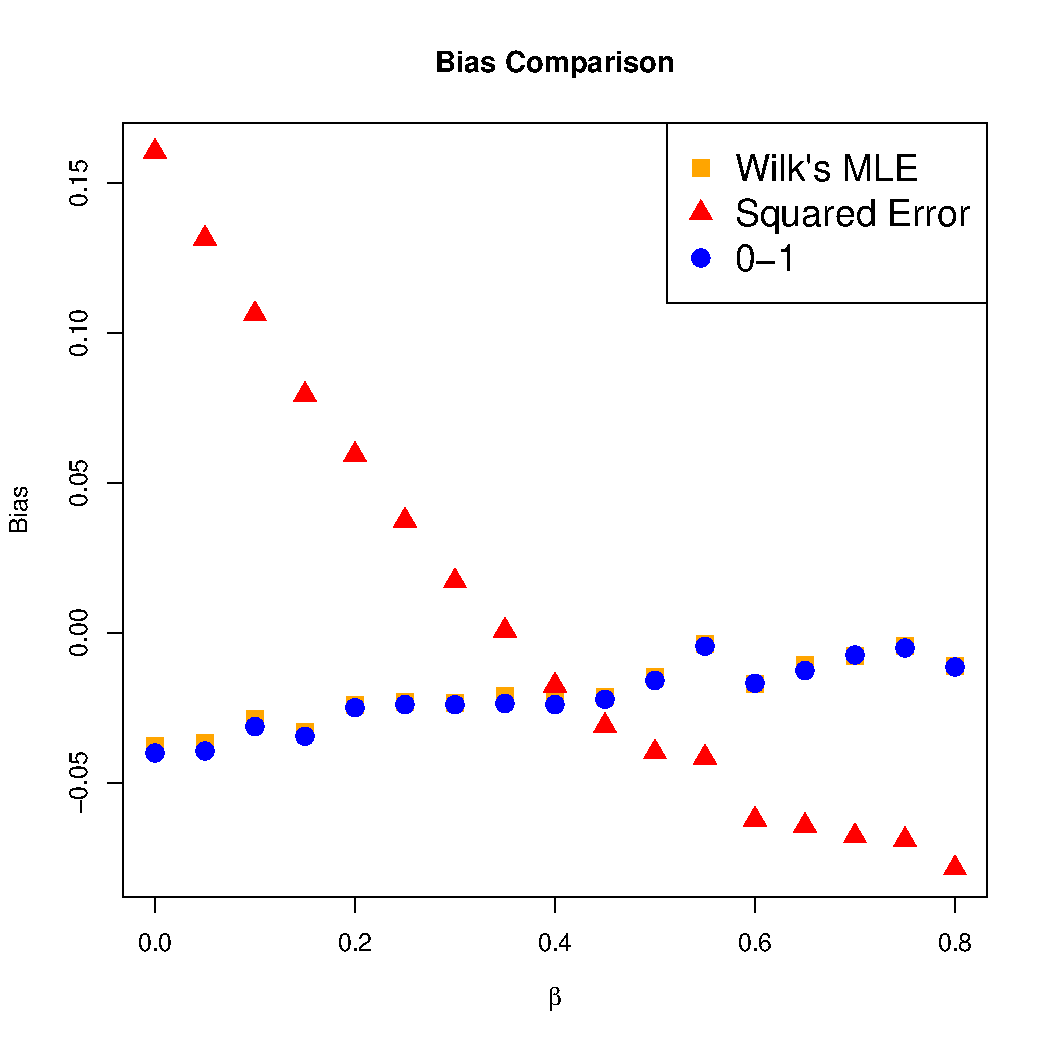
\includegraphics[scale=.45]{bias.pdf}
\end{center}

It would appear that the Wilk's method for MLE estimation, and squared-error loss gives similar MSE, while keeping a relatively stable bias. This may be helpful as we further use, and estimate the Poisson regression. 


\closing{Sincerely,}
\end{letter}
\end{document}
